% !TEX encoding = UTF-8
% !TEX TS-program = pdflatex
% !TEX root = ../thesis.tex

%**************************************************************
\chapter{METODOLOGIA}
\label{Capitolo3}
\thispagestyle{empty}

Nel capitolo precedente sono stati spiegati tutti i concetti principali che 
compongono un sistema di visione artificiale, il quale ha lo scopo principale 
di effettuare la comprensione della scena mediante l'utilizzo di tecniche di 
object detection e di semantic segmentation. Oltre a questi concetti, sono 
state definite anche le comuni tecniche di compressione/ottimizzazione che 
permettono ad un modello di essere eseguito anche su dispositivi a limitate 
risorse computazionali, relativamente economico, alla portata di tutti. 
L'obiettivo finale dello studio è basato sull'incremento delle prestazioni di 
un modello tramite l'utilizzo di una delle tecniche di compressione/ottimizzazione 
citate nel capitolo precedente. Nel seguente capitolo vengono 
riportate tutte le metodologie adottate che hanno portato alla realizzazione 
di un metodo personalizzato avente lo scopo prefissato. Il focus principale 
sarà rivolto verso la tecnica di object detection. È proprio quest'ultima 
tecnica ad essere stata utilizzata maggiormente in questo elaborato. Le
risorse computazionali richieste da codesta risultano essere onerose. Essendo 
un sistema autonomo implementato all'interno di una centralina dedicata, 
bisogna aver un chiaro prospetto delle potenzialità richieste da un modello di 
visione artificiale per poter raggiungere l'obiettivo finale. Il dispositivo preso 
in riferimento è costituito da un nota scheda di elaborazione embedded, che 
prende il nome di Nvidia Jetson Nano. Le potenzialità messe a disposizione 
da questa scheda sono state comparate, in termini di Frames-per-Second 
(FPS), con quelle messe a disposizione sia dal computer del sottoscritto 
che da Google Colaboratory (Colab). Avendo caratteristiche hardware ben 
differenti l'uno dall'altro, si è pensato di creare una comparazione standard 
composta dallo stesso codice eseguito su tutte e tre le diverse architetture. 
Dopo aver ottenuto i primi risultati dai modelli pre-addestrati, messi gentilmente 
a disposizione da NVidia, questi hanno costituito le baselines ovvero 
i punti di riferimento da cui partire. Per la visualizzazione dei risultati 
ottenuti in ogni test, si rimanda la lettura al capitolo (\ref{Chapter4}).

\section{NVidia Jetson Nano}
La Jetson Nano (B01), presentata nel Marzo del 2019,  è una scheda embedded 
sviluppata da NVidia che rappresenta il prodotto più piccolo della 
famiglia Jetson. L'utilizzo della scheda è rivolto principalmente verso varie 
applicazioni di intelligenza artificiale, visione artificiale e robotica. A bordo 
troviamo un processore e una scheda madre che offre una potenza di calcolo 
pari a 128 Cuda cores. L'obiettivo di questa scheda è quello di funzionare 
con reti neurali e offrire le migliori prestazioni quando viene utilizzata per 
eseguire inferenze. A differenza di altre architetture, lo Jetson Nano utilizza 
una precisione Floating point (FP) a 16-bit che lo rende competitivo rispetto 
ad altri device embedded. Purtroppo non supporta la precisione a 8-bit 
ma è comunque in grado di lavorare con qualsiasi rete disponibile e con 
qualsiasi framework di deep learning popolare (es: Pytorch, TensorFlow, 
Keras, Caffe etc.). In questo dispositivo è possibile effettuare sia il rilascio 
(deploy) dell'applicazione che l'addestramento della rete ma, in quest'ultimo 
caso, risulta essere lento a causa delle prestazioni computazionali ridotte. 
Risulta inoltre possibile effetuare operazioni di transfer learning tra i modelli.
Oltre ad avere il vantaggio delle dimensioni ridotte, un altro principale vantaggio 
della Jetson Nano deriva dall'applicazione dell'acceleratore TensorRT. 
Quest'ultimo esegue un processo di quantizzazione che è utile a convertire i 
pesi e gli input in precisioni Floating Point inferiori, in modo da preservare 
la memoria che, su una scheda del genere, rappresenta una limitazione. A 
tal proposito, il dispositivo non fornisce alcun tipo di memoria integrata, 
ma esiste la possibilità di aggiungerne una grazie alla presenza di uno slot 
di espansione in cui è possibile alloggiare una scheda micro-sd. Essendo una 
scheda embedded, a differenza di altri computer che utilizzano alimentatori 
da diversi Watts (W), la Jetson Nano può utilizzare due diversi livelli di 
wattaggio. Il primo, quello da 5W, raggiungibile grazie alla presenza di 
una porta micro-usb, mentre il secondo, quello da 10W, è raggiungibile solo 
grazie all'utilizzo di un alimentatore esterno collegato tramite l'ingresso 
jack. Il massimo livello di performance, raggiungibile dalla GPU, avviene 
proprio tramite l'utilizzo dell'alimentatore esterno. Per rendere l'idea delle 
dimensioni e dell'intera architettura, in Figura (\ref{jetson}) è riportata la Jetson 
Nano.
\begin{figure}[]
    \begin{minipage}[t]{.45\textwidth}
        \centering
        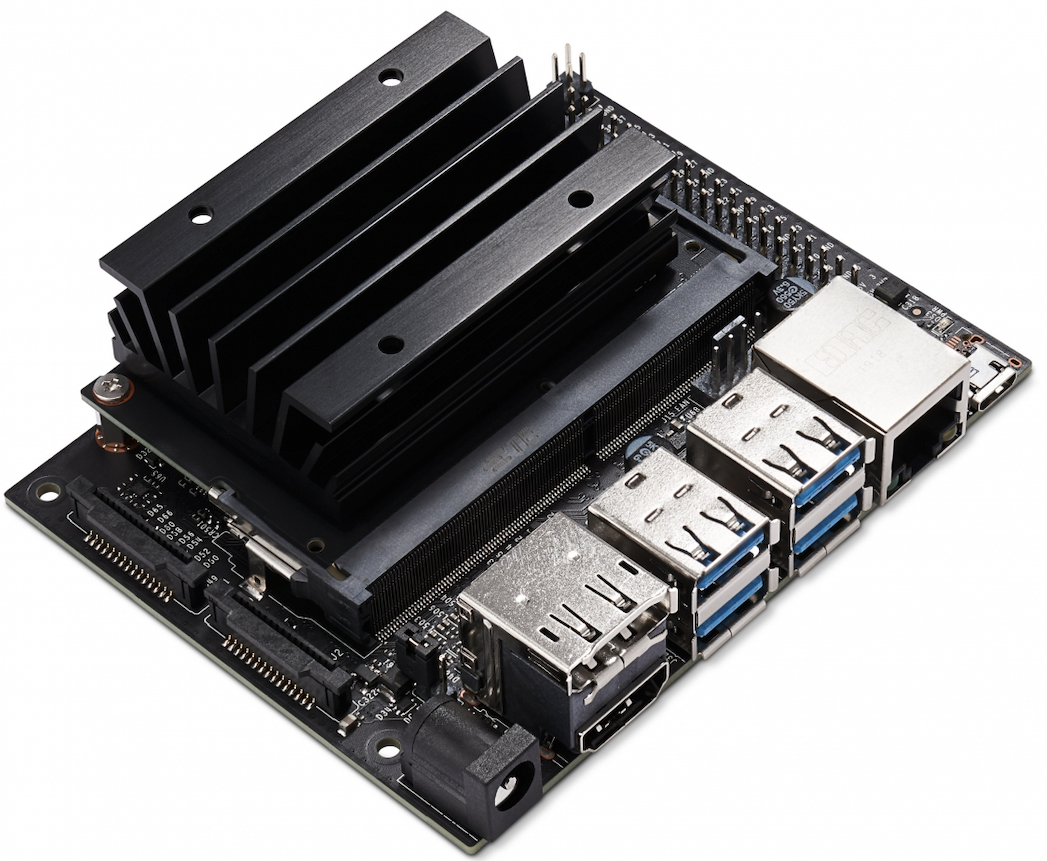
\includegraphics[width=\textwidth]{jetson1.png}
    \end{minipage}
    \hfill
    \begin{minipage}[t]{.45\textwidth}
        \centering
        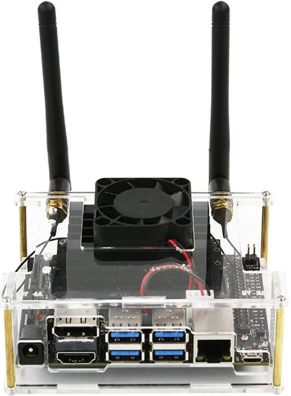
\includegraphics[width= 0.8\textwidth]{jetson2.png}
    \end{minipage}  
    \caption{NVidia Jetson Nano.}
    \label{jetson}
\end{figure}

\section{Test Frameworks}
\subsection{TensorRT}
\begin{figure}
    \centering
    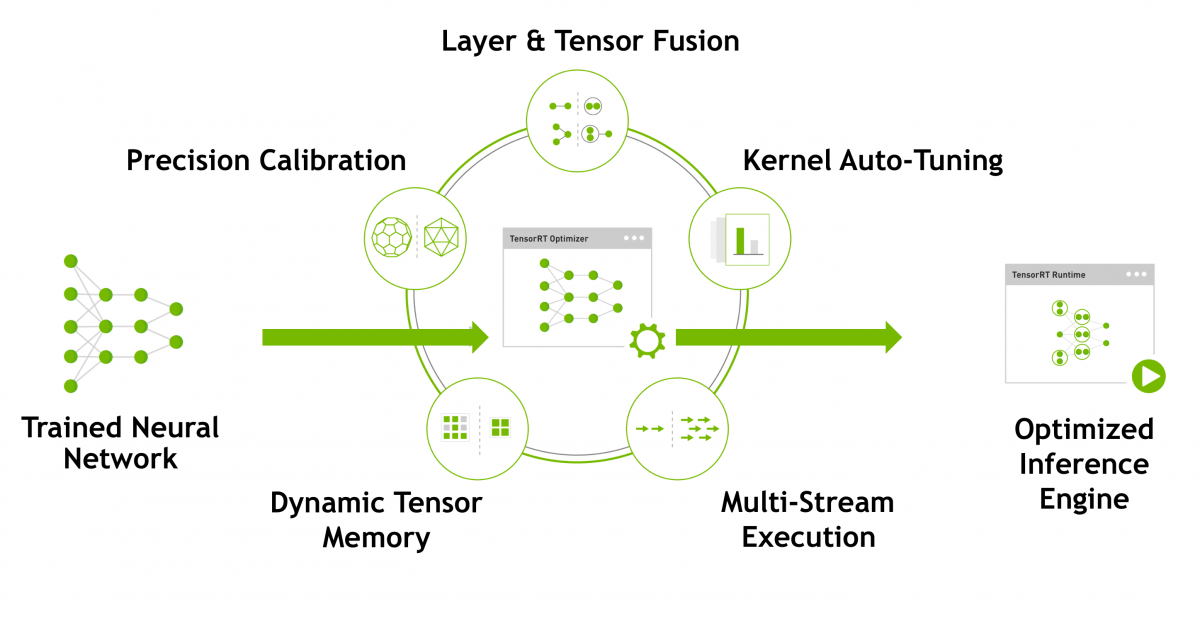
\includegraphics[width = \linewidth]{tensorrtOpt.png}
    \centering
    \caption{Ottimizzazioni si TensorRT sui modelli.}
    \label{tensorrt}
\end{figure}
TensorRT è un framework di machine learning, sviluppato interamente da 
NVidia, che esegue cinque diverse procedure di ottimizzazione su architetture 
basate su scheda GPU NVidia (Fig. (\ref{tensorrt})). 
\begin{enumerate}
    \item {\bfseries{\emph{Precision Calibration}}}: in questa ottimizzazione viene eseguita 
    l'operazione di \emph{Quantizzazione} che permette di mappare tutti i valori 
    dei pesi da una precisione FP32 bit a FP16 bit, creando una perdita 
    di precisione trascurabile.
    \item {\bfseries{\emph{Layer \& Tensor Fusion}}}: la seconda ottimizzazione riguarda l'eliminazione 
    di tutti quei layer che non vengono utilizzati, questo è 
    utile per poter evitare calcoli inutili. Successivamente, le operazioni 
    di Convoluzione, ReLU e normalizzazione Batch, vengono fuse in un 
    unico layer (\emph{CBR}). Questa operazione permette di eseguire calcoli 
    in una maniera più veloce ed efficace. Nella Figura (\ref{fusion_tensorrt}) si possono 
    vedere meglio quali sono tutti i layer che vengono fusi da TensorRT.
    \item {\bfseries{\emph{Kernel Auto-Tuning}}}: la terza ottimizzazione viene effettuata direttamente 
    sui filtri utilizzati nella rete. Durante questa fase vengono 
    selezionati i migliori layer, algoritmi e dimensioni di batch in base alla 
    piattaforma GPU di destinazione.
    \item {\bfseries{\emph{Dynamic Tensor Memory}}}: la gestione della memoria viene effettuata 
    proprio in questa ottimizzazione. TensorRT alloca memoria 
    solo per durante il periodo di vita di un tensore scongiurando un 
    sovraccarico di allocazioni permettendo esecuzioni rapide ed efficienti.
    \item {\bfseries{\emph{Multiple Stream Execution}}}: l'ultima ottimizzazione riguarda l'elaborazione 
    parallela di multipli flussi di input. Fondamentalmente, 
    questo è possibile utilizzando la libreria CUDA stream.
\end{enumerate}
L'aspetto più importante da ricordarsi, quando si utilizza TensorRT, è che 
bisogna assicurarsi che la procedura di ottimizzazione avvenga sulla stessa 
GPU NVidia che verrà utilizzata per l'inferenza. Questo deve avvenire 
in quanto TensorRT utilizza kernel specifici a seconda della piattaforma 
di destinazione. L'utilizzo di una ottimizzazione su una differente scheda 
grafica porta alla creazione di errori in fase di inferenza. 
\begin{figure}
    \centering
    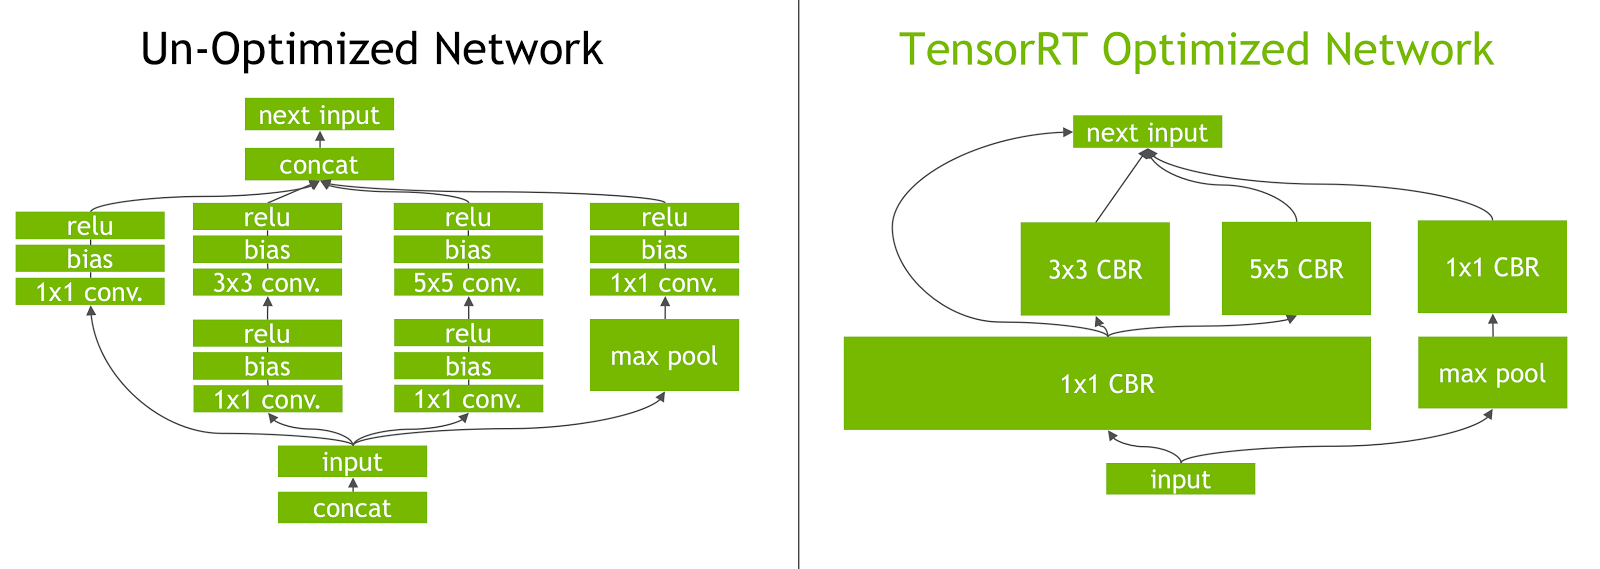
\includegraphics[width = \linewidth]{optTensor.png}
    \centering
    \caption{Fusione dei livelli Convolutional, Batch e ReLU eseguita da TensorRT.}
    \label{fusion_tensorrt}
\end{figure}

\subsection{NVidia Jetson utils}\label{utils}
NVidia dispone di una comunità che supporta l'evoluzione di tutte le sue schede 
embedded, inclusa la Jetson Nano. Questa associazione ha dato vita 
a delle librerie utilizzate in ambito di computer vision, nello specifico rivolto 
alla gestione e alla  progettazione di reti neurali. In ambito di inferenza, una 
parte di codeste utilizza l'acceleratore TensorRT per distribuire in modo 
efficiente le reti neurali sulla piattaforma Jetson utilizzata, consentendo 
un miglioramento delle prestazioni e al contempo una migliore efficienza 
energetica. Il codice sorgente messo a disposizione, sviluppato sia in linguaggio 
C++ che in Python (principalmente utilizzato in questo elaborato), 
è composto da diversi scripts che mirano ad eseguire i modelli per svolgere 
svariate attività:
\begin{itemize}
    \item \emph{ImageNet.py}: per attività di Image Recognition;
    \item \emph{DetectNet.py}: per attività di Object detection;
    \item \emph{SegNet.py}: per attività di Semantic Segmentation;
    \item \emph{PoseNet.py}: per attività di Pose Estimation.
\end{itemize}
Ognuno di questi ha lo scopo di eseguire l'inferenza di una apposita rete 
per produrre l'output inerente una specifica attività. In questa tesi sono 
stati utilizzati i primi tre scripts in quanto coerenti con lo scopo prefissato. 
L'input è costituito da uno stream di immagini, video o dati, proveniente 
da una sorgente esterna come per esempio una webcam esterna, collegata 
tramite una porta usb, oppure una webcam collegata tramite interfaccia 
CSI/ISP predisposta direttamente sulla scheda. I frame di input possono 
provenire da un file avente estensione jpeg, mp4, RTP, RTPS etc. Nel caso 
in cui l'input provenga da una fonte esterna, verrà utilizzato il protocollo 
V4L2 che imposterà il maggior numero di frame rate alla massima risoluzione 
supportata dalla fonte. Per quanto riguarda l'output, questo può 
essere distribuito nel medesimo formato di input. I codecs supportati dalla 
piattaforma sono i seguenti:
\begin{itemize}
    \item \emph{Decode}: H.264, H.265, VP8, VP9, MPEG-2, MPEG-4 e MJPEG;
    \item \emph{Encode}: H.264, H.265, VP8, VP9 e MJPEG.
\end{itemize}
Le APIs mettono a disposizione anche alcuni scripts che utilizzano il supporto 
CUDA in grado di gestire e manipolare le immagini, che siano di input o 
di output. Ritornando agli scripts principali, ImageNet accetta un'immagine 
in input e restituendone un intervallo di probabilità in output per ogni classe. 
DetectNet, a differenza di ImageNet, oltre a permette di concentrarsi sul rilevamento 
di oggetti, specifica la loro posizione tramite delle bounding boxes, 
all'interno del frame in input. Rispetto alla classificazione delle immagini, 
le reti utilizzate in questo contesto sono in grado di rilevare multipli oggetti, 
appartenenti alla stessa categoria e non, nell'input specificato. L'output 
prodotto è rappresentato da delle coordinate utili a delimitare i riquadri che 
contraddistinguono ogni singolo oggetto di ogni classe (Fig. \ref{detectnet_result}).
\begin{figure}
    \centering
    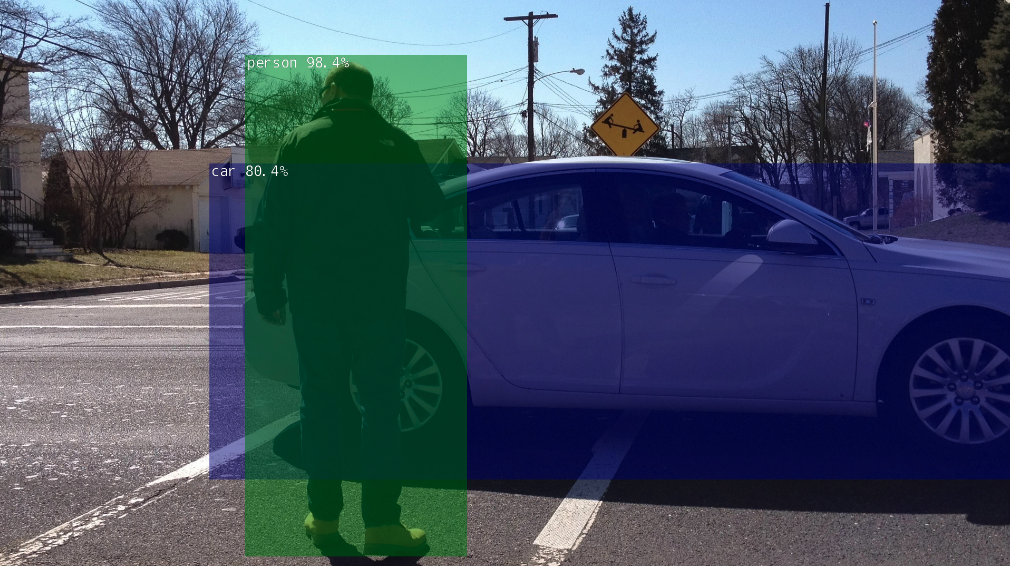
\includegraphics[width = \linewidth]{detectnet_result.png}
    \centering
    \caption{Esempio di ouput prodotto da DetectNet sulla Jetson Nano.}
    \label{detectnet_result}
\end{figure}
Per quanto 
riguarda l'attività di segmentazione semantica, questa viene interamente 
svolta dallo script Python Segnet. L'output prodotto da quest'ultimo si 
basa in un'immagine in cui vi è applicata una maschera sovrapposta utile a 
classificare ogni singolo pixel presente nell'immagine di input. Ogni pixel 
della maschera corrisponderà alla classe dell'oggetto sottostante classificato 
(Fig. \ref{segnet_result}).
\begin{figure}
    \centering
    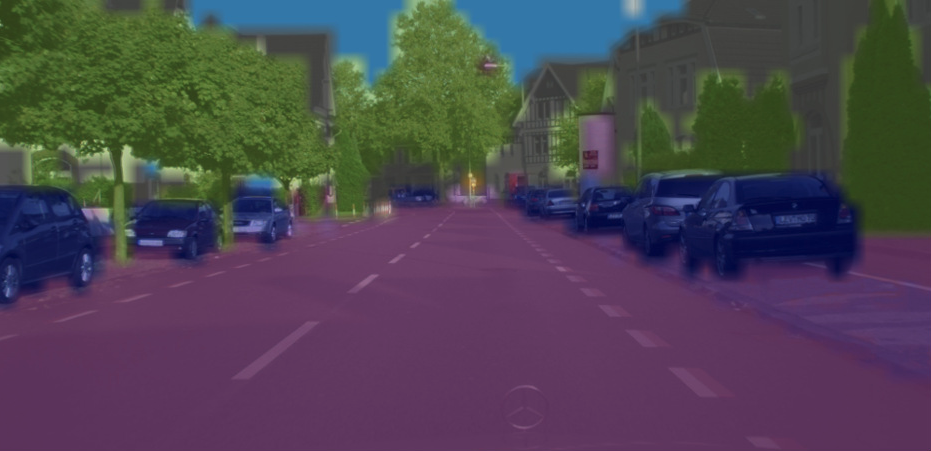
\includegraphics[width = \linewidth]{segnet_result.png}
    \centering
    \caption{Esempio di ouput prodotto da SegNet sulla Jetson Nano.}
    \label{segnet_result}
\end{figure}
Seppur non consigliata come piattaforma su cui effettuare il 
training di un modello, nella repository ufficiale \cite{repo_jetson_nano} viene riportato un link ad 
un'altra repository \cite{repo_pytorch_training} contenente il codice sorgente utile ad addestrare tutti 
i modelli impiegati nelle varie attività. Esiste una documentazione ufficiale 
contenente tutte le informazioni riguardanti gli script citati utilizzabili in 
ogni architettura presente nella famiglia Jetson \cite{Documentation_jetson}. Sia nel training che 
nell'inferenza di ogni modello, il framework di ML utilizzato è Pytorch.


\section{Frames-per-Second (FPS)}
La velocità di inferenza rappresenta un indicatore di performance di ogni 
modello. Per poterla calcolare, la velocità di inferenza è rappresentata dai 
\emph{Frames-per-Second (FPS)} (\ref{FPS_Count}):
\begin{equation}\label{FPS_Count}
    FPS = \frac{1}{Ending \ Time - Starting \ Time}
\end{equation}
Questa misura è variabile e serve per rappresentare tre diversi elementi:
\begin{itemize}
    \item {\bfseries{\emph{Input}}}: ogni rete prende in input una sequenza di frame appartenenti 
    a un video/immagini. Ogni sequenza può avere un numero di FPS variabile. In 
    questo elaborato, vengono testati diversi video a 30FPS e a 60FPS.
    \item {\bfseries{\emph{Netwrok}}}: la velocità che la rete impiega ad effettuare uno specifico 
    task, può essere rappresentata dal numero di FPS. Riconoscere e/o 
    segmentare un oggetto appare essere un'attività onerosa in termini 
    computazionali, pertanto una rete è considerata veloce se, oltre a 
    produrre un output adeguato, svolge ogni task in un tempo breve.
    \item {\bfseries{\emph{Output}}}: il risultato prodotto da una rete è visibile solamente a 
    schermo. I video/immagini mostrati/e hanno una velocità di riproduzione 
    che è influenzata dal numero di FPS.
\end{itemize}
Tra le API messe a disposizione da NVidia, citate nella sezione \ref{utils}, 
fondamentale è risultato l'utilizzo dei metodi incaricati di calcolare la 
velocità d'inferenza, di input e di output raggiunta da ogni modello su ogni 
attività richiesta. 